%%%%%%%% ICML SUBMISSION -- Learned Specific Epistasis (story C) %%%%%%%%
\documentclass{article}

\usepackage{microtype}
\usepackage{graphicx}
\usepackage{subcaption}
\usepackage{booktabs}
\usepackage{multirow}
\usepackage{xcolor}
\usepackage{hyperref}
\newcommand{\theHalgorithm}{\arabic{algorithm}}
\usepackage{icml2025}
\usepackage{amsmath}
\usepackage{amssymb}
\usepackage{mathtools}
\usepackage{amsthm}
\usepackage{algorithm}
\usepackage{algorithmic}
\usepackage[capitalize,noabbrev]{cleveref}

\graphicspath{{./figures_epistasis/}}

\newcommand{\eps}{\varepsilon}
\newcommand{\E}{\mathbb{E}}
\DeclareMathOperator{\spearman}{\rho}

\icmltitlerunning{Learned Specific Epistasis for Protein Function}

\begin{document}

\twocolumn[
  \icmltitle{Learned Specific Epistasis: Predicting and Designing Functional\\
  Protein Interactions Invisible to Zero-Shot Language Models}

  \icmlsetsymbol{equal}{*}
  \begin{icmlauthorlist}
    \icmlauthor{Anonymous Authors}{anon}
  \end{icmlauthorlist}
  \icmlaffiliation{anon}{Anonymous Institution}
  \icmlcorrespondingauthor{Anonymous}{anon@anon.org}
  \icmlkeywords{protein language models, epistasis, protein design, deep mutational scanning, fitness landscapes}
  \vskip 0.3in
]

\printAffiliationsAndNotice{}

\begin{abstract}
Multi-mutant protein fitness is not the sum of its parts. We decompose
multi-mutant landscapes into three layers: an \emph{additive} baseline (the sum
of single-mutant effects), \emph{global epistasis} (a monotonic saturation link
imposed by the assay), and \emph{specific epistasis} (the residue-pair
interaction that remains). On the Megascale double-mutant stability corpus
(149 protein domains, 131{,}062 double mutants) the additive baseline is worse
than predicting the mean for 72\% of proteins (median $R^2=-0.91$), a per-protein
monotonic link recovers most of the gap (median $R^2=0.72$), and the leftover
specific epistasis is large and ubiquitous (median residual std $0.42$ kcal/mol;
$\geq 10\%$ of double-mutant variance in 98\% of proteins). We then make and test
a sharper claim about \emph{function}: specific epistasis in functional assays
(binding, fluorescence) is real, is \emph{invisible} to zero-shot protein
language models, yet is \emph{predictable} from the internal representations of a
diffusion protein language model (DPLM). A trained pairwise coupling head over
DPLM representations predicts held-out functional epistasis far above the
zero-shot pseudo-likelihood floor, and ranking candidate double mutants by
predicted epistasis recovers gain-of-function combinations that the additive
model structurally cannot find. Fine-tuning DPLM end-to-end with LoRA across the 149 Megascale stability
domains shows the same epistasis-prediction skill transfers across proteins:
on 25 held-out domains that contribute no training examples it reaches a median
Spearman of $0.33$, above the $0.25$ zero-shot DPLM pseudo-likelihood reference on
the same stability task. All claims are backed
by held-out evaluations on real deep-mutational-scanning data.
\end{abstract}

\section{Introduction}
\label{sec:intro}

Engineering a protein almost always requires \emph{combining} mutations.
Yet the effect of a combination is rarely the sum of the parts: substitutions
interact, an effect known as epistasis. Two forms are usually conflated.
\emph{Global} (or nonspecific) epistasis is a smooth, monotonic distortion that
acts on every variant the same way -- a brightness threshold for a fluorescence
assay, a folding-stability floor, a saturating dose-response -- and is fully
explained by the additive prediction passed through a single nonlinear link
\citep{otwinowski2018inferring,sailer2017detecting}. \emph{Specific} epistasis
is what remains: an interaction tied to a particular pair (or set) of residues,
the part of the landscape that a sum-of-singles model, even after correcting for
any global nonlinearity, cannot represent.

Specific epistasis is exactly where combinatorial protein design either wins or
fails, because it is the only part of the landscape under which a combination can
beat the additive expectation. It is also the part that current pretrained
protein language models (PLMs) are weakest at. Zero-shot PLM scores
\citep{meier2021language,wang2024dplm} are trained on natural sequence
statistics, which track folding stability and evolutionary conservation but carry
little information about an arbitrary laboratory \emph{function} assay. The
emerging consensus that ``PLMs capture epistasis'' is, we argue, largely a
statement about \emph{global} epistasis on \emph{stability}; it does not transfer
to specific epistasis on function.

This paper makes one claim and supports it with held-out experiments:

\begin{quote}
\emph{Specific epistasis in protein function is real, is invisible to zero-shot
protein language models, but is predictable from a PLM's internal
representations -- enough to design gain-of-function combinations that additive
models structurally cannot find.}
\end{quote}

Our contributions are:
\begin{itemize}
  \item \textbf{A three-layer decomposition} (\cref{sec:decomp}) that separates
  additive, global, and specific epistasis per protein, and a measurement of how
  large and how widespread specific epistasis is across 149 protein domains
  (\cref{sec:results-decomp}).
  \item \textbf{Model 1 (predict)} (\cref{sec:model1}): a pairwise coupling head
  over DPLM-650M representations that predicts held-out specific epistasis on
  functional assays, far above the zero-shot pseudo-likelihood floor, while never
  seeing residue indices -- so the signal is genuinely in the representation.
  \item \textbf{Model 2 (design)} (\cref{sec:model2}): ranking candidate double
  mutants by predicted epistasis recovers gain-of-function combinations among
  additively-mediocre candidates, with a matched-additive control that isolates
  the part of the signal the additive model cannot see.
  \item \textbf{Cross-protein generalization} (\cref{sec:e2e}): an end-to-end
  LoRA fine-tune of DPLM that transfers learned epistasis to 25 held-out
  Megascale stability domains (median Spearman $0.33$, above the $0.25$ corpus-level
  zero-shot DPLM PLL reference), showing the skill is not memorized per protein. This cross-protein
  test runs on the stability corpus because it is the only corpus here with
  enough proteins for a held-out-\emph{protein} split.
\end{itemize}

\section{Related work}
\label{sec:related}

\paragraph{Global epistasis.}
A long line of work models multi-mutant fitness as a monotonic nonlinearity
applied to a latent additive trait
\citep{otwinowski2018inferring,sailer2017detecting}. Inferring and removing this
link is now standard practice and explains much of the apparent non-additivity in
deep mutational scans. Our decomposition uses a per-protein monotonic (isotonic)
link as the global layer, and defines specific epistasis as the residual after
both the additive and global layers, so that any held-out skill on it is genuine
pairwise interaction by construction.

\paragraph{Zero-shot PLMs and epistasis.}
Protein language models predict variant effects zero-shot from sequence
likelihood \citep{meier2021language,wang2024dplm,lin2023esm2}, and recent work
argues they implicitly encode epistasis. We separate the claim: PLM
pseudo-likelihood tracks the \emph{global}, stability-coupled component, but its
zero-shot epistasis signal is weak even on stability and is expected to be near
zero on functional assays (\cref{sec:results-zs}). This motivates a \emph{trained}
read-out rather than a zero-shot score.

\paragraph{Assay-labeled models.}
Combining PLM representations with assay labels improves fitness prediction
\citep{hsu2022learning}. We focus this idea on the specific-epistasis residual
rather than raw fitness, which makes the target a clean test of interaction
modeling and removes the additive and global components that PLMs already explain.

\paragraph{Generative and guided protein design.}
A parallel line designs sequences \emph{generatively}, steering a diffusion or
flow model toward a reward: classifier-style guidance for discrete state spaces
\citep{gruver2023protein,nisonoff2025unlocking}, reward fine-tuning of discrete
diffusion models \citep{wang2025drakes}, and derivative-free value-based decoding
\citep{li2024svdd}. These methods \emph{propose} new variants and are scored by a
(often learned or in-silico) reward. Our Model 2 is deliberately not generative:
it is a ranking policy over a pool of \emph{already measured} combinations, so
every selected design carries a ground-truth label and no reward model can be
gamed. We therefore treat guided generation as related context rather than a
matched baseline for the ranking claim, and benchmark the best-of-$N$ reranking
reduction that does apply to a closed measured pool (\cref{sec:results-model2}).

\paragraph{Datasets.}
We use the Megascale stability corpus \citep{tsuboyama2023mega} for the
stability decomposition and ProteinGym \citep{notin2023proteingym} functional
assays -- GB1 binding \citep{olson2014comprehensive,wu2016adaptation} and GFP
fluorescence \citep{sarkisyan2016local} -- for the functional claims. We adapt
DPLM \citep{wang2024dplm} with LoRA \citep{hu2022lora}.

\section{Problem setup and the three-layer decomposition}
\label{sec:decomp}

Let $y(x)$ be the measured fitness of variant $x$ relative to wildtype, and let
$s_i$ be the measured effect of single mutation $i$. For a multi-mutant $x$ that
combines mutations in a set $S$, define the three layers:
\begin{align}
  \underbrace{a(x)}_{\text{additive}} &= \sum_{i \in S} s_i, \\
  \underbrace{g(x)}_{\text{global}}   &= \phi\!\big(a(x)\big), \\
  \underbrace{\eps(x)}_{\text{specific}} &= y(x) - g(x),
\end{align}
where $\phi$ is a per-protein monotonic link fit by isotonic regression on the
$\big(a(x), y(x)\big)$ pairs. The additive layer is parameter-free given the
single-mutant map; the global layer adds one monotonic curve per protein; the
specific layer is the residual. By construction, $\eps(x)$ contains no additive
or smooth-saturation signal, so a model that predicts $\eps$ on held-out
combinations has learned genuine pairwise interaction, not a re-scaled additive
effect (the same negative-control logic as high-order epistasis audits,
\citealp{sailer2017detecting}).

We quantify each protein by the variance of measured fitness explained by the
additive baseline ($R^2_{\text{add}}$) and by the additive$+$global model
($R^2_{\text{glob}}$), and the specific epistasis by the standard deviation of
$\eps$ and its share of double-mutant variance. The implementation lives in
\texttt{src/phaseagent/epistasis\_decomposition.py} and the committed per-protein
table in \texttt{outputs/epistasis/decomposition\_atlas.csv}.

\section{Model 1: predicting specific epistasis from DPLM representations}
\label{sec:model1}

Model 1 predicts the specific-epistasis residual $\eps_{ij}$ of a double mutant
at positions $i,j$ from a frozen DPLM-650M. Let $H \in \mathbb{R}^{L \times d}$ be
the last-layer hidden states of the wildtype sequence. We take the
representations $H_i, H_j$ at the two mutated positions, project them, and form a
bilinear coupling feature $\text{proj}(H_i) \odot \text{proj}(H_j)$, concatenated
with amino-acid identity embeddings of the two substitutions and the zero-shot
DPLM pseudo-log-likelihood (PLL) epistasis
\begin{equation}
  \label{eq:zs}
  \eps^{\text{zs}}_{ij} = \text{LL}(x_{ij}) - \text{LL}(x_i) - \text{LL}(x_j) + \text{LL}(x_{\text{wt}})
\end{equation}
as a residual base, where $\text{LL}(x)$ is DPLM's sequence pseudo-log-likelihood
(the residue log-probabilities summed over the sequence). A small head regresses $\eps_{ij}$. Crucially, the head never
receives position indices $i,j$ -- only representations and amino-acid identities
-- so any predictive skill comes from the representation, not from memorizing
which positions interact. We additionally test \emph{representation-shift}
features $H^{(i\to a)}_j - H^{\text{wt}}_j$, the change DPLM predicts at $j$ when
$i$ is mutated, which directly probe the model's internal coupling.

We evaluate Model 1 in two held-out regimes (\cref{sec:exp}): held-out
\emph{doubles} (complete a combinatorial landscape from a partial scan at known
coupled positions -- the realistic design setting) and held-out \emph{positions}
(transfer to position pairs never seen in training -- a strictly harder
cross-position test). Code: \texttt{scripts/train\_model1.py}.

\section{Model 2: epistasis-aware design}
\label{sec:model2}

The design task is to pick gain-of-function combinations from a pool where the
additive model is uninformative. Among GB1 double mutants whose two singles are
individually mediocre, the additive prediction rates all candidates roughly
equal; only specific epistasis distinguishes a synergistic pair from an
antagonistic one. Model 2 ranks these candidates by predicted specific epistasis
(from Model 1) and selects the top fraction.

We report two quantities. (i) \emph{Gain-of-function recovery}: the measured
function of the selected variants versus the additive pool mean, versus the
oracle top-selection, and versus a \emph{best-of-$N$ rerank} that scores the same
pool with the zero-shot DPLM PLL epistasis (the standard PLM-as-reward design
baseline). (ii) The \emph{matched-additive control}: within narrow bins of
additive prediction (so additive value is held fixed), the rank correlation
between predicted and measured specific epistasis. A positive within-bin
correlation is, by construction, signal that the additive model cannot access.
Code: \texttt{scripts/model2\_design.py}. Because every generated GB1 combination
is measurable in the complete combinatorial assay
\citep{olson2014comprehensive,wu2016adaptation}, this is a closed evaluation: no
selected design is unscored.

\section{Cross-protein generalization: end-to-end LoRA fine-tune}
\label{sec:e2e}

Models 1 and 2 are trained per assay. To test whether learned epistasis
\emph{transfers across proteins}, we fine-tune DPLM-650M end-to-end with LoRA
(rank 64, adapters on the attention query/value projections) together with a
pairwise epistasis head on the Megascale stability corpus -- the only corpus
here with enough proteins (149 domains) for a held-out-\emph{protein} split --
trained on the double mutants of $\sim$120 domains and evaluated on $\sim$25
\emph{held-out domains} that contribute no training examples. The headline metric is the median per-held-out-protein Spearman
correlation between predicted and measured specific epistasis. Per-protein
targets are standardized before subsampling (with \texttt{ddof}$=0$). The run is
defined in \texttt{modal\_app\_v2.py::train\_epistasis\_e2e}; its committed
artifact is \texttt{outputs/epistasis/e2e\_results.json}.

\section{Experiments}
\label{sec:exp}

\paragraph{Data.}
Stability decomposition: Megascale dataset2 \citep{tsuboyama2023mega}, the curated
double mutants over 149 natural and de novo domains. Functional assays from
ProteinGym v1.3 \citep{notin2023proteingym}: GB1 IgG-binding (Olson, complete
pairwise; Wu, four-site combinatorial)
\citep{olson2014comprehensive,wu2016adaptation} and GFP fluorescence (Sarkisyan)
\citep{sarkisyan2016local}. All splits are held-out; targets are the
specific-epistasis residual defined in \cref{sec:decomp}.

\paragraph{Baselines.}
(i) \emph{Additive}: the sum-of-singles prediction, the structural null for any
epistasis claim. (ii) \emph{Zero-shot DPLM PLL}: \cref{eq:zs}, the pretrained-PLM
epistasis score with no task labels. (iii) For design, \emph{best-of-$N$
reranking} of randomly drawn candidates and an additive-ranking control. Stronger
generative comparators -- discrete-diffusion guidance
\citep{gruver2023protein,nisonoff2025unlocking} and reward-guided refinement
\citep{wang2025drakes,li2024svdd} -- are required only if a generative design claim
is made; our Model 2 is a ranking policy over measurable candidates, so the
additive and best-of-$N$ controls are the matched baselines.

\paragraph{Metrics.}
Variance explained ($R^2$) for the decomposition; Spearman rank correlation
between predicted and measured specific epistasis for Models 1 and the e2e
fine-tune (per protein, then median across proteins); gain-of-function recovery
and within-additive-bin Spearman for Model 2.

\paragraph{Implementation details.}
Model 1's coupling head projects each mutated-position DPLM-650M hidden state
($d=1280$) to $128$ dimensions, forms the bilinear product
$\text{proj}(H_i)\odot\text{proj}(H_j)$, and concatenates $16$-dimensional
embeddings of the four amino-acid identities (wild-type and mutant at both sites)
with the $z$-scored zero-shot PLL feature; a LayerNorm followed by a
two-hidden-layer MLP ($256$ then $128$ units, GELU, dropout $0.3$) regresses the
specific-epistasis residual, with a learnable scalar gain on the PLL term as a
residual base. The held-out-position variant additionally consumes the
representation-shift features (\cref{sec:model1}). We optimize with AdamW
(learning rate $2\times10^{-3}$, weight decay $10^{-4}$) for $200$ epochs at batch
size $1024$ under a Huber (smooth-$L_1$) loss on per-fold-standardized targets.
The held-out-doubles split is $5$-fold shuffled cross-validation; the
held-out-position split is $5$-fold grouped cross-validation keyed on residue
position, so no test pair's positions appear in training. All features are
$z$-scored per dimension, and the head never receives position indices. Full
configuration: \texttt{scripts/train\_model1.py}.

\section{Results}
\label{sec:results}

\subsection{The three-layer decomposition of stability}
\label{sec:results-decomp}

\Cref{fig:three_layer} summarizes the decomposition over the 149 Megascale
domains. The additive baseline is \emph{worse than predicting the mean} for 72\%
of proteins (median $R^2_{\text{add}}=-0.91$): summing single-mutant effects
systematically overshoots, because the stability assay saturates at a floor.
Passing the additive prediction through a single per-protein monotonic link
recovers most of the gap, lifting the median variance explained to
$R^2_{\text{glob}}=0.72$. This is the global-epistasis layer, and it is well
captured by a parameter-light saturation curve.

What remains -- specific epistasis -- is not noise. \Cref{fig:specific} shows the
distribution of the per-protein residual standard deviation: the median is
$0.42$ kcal/mol and it exceeds $0.3$ kcal/mol for 85\% of proteins. Specific
epistasis accounts for at least 10\% of double-mutant variance in 98\% of proteins
(median share 28\%): it is real explained variance, not measurement scatter.
Specific epistasis is therefore both large and ubiquitous: a real,
widespread signal that an additive-plus-global model leaves entirely on the
table. These numbers are computed by
\texttt{scripts/build\_decomposition\_artifact.py} from the committed atlas and
are listed in \cref{tab:decomp}. Bootstrapping the 149 proteins ($2{,}000$
resamples) confirms each headline median is robust to protein sampling and that
all three decomposition claims exclude their null: the additive $R^2$ median is
$-0.91$ (95\% CI $[-1.39, -0.58]$, entirely below zero -- the additive baseline
is worse than the mean for the typical protein), the $+$global median is $0.72$
($[0.67, 0.74]$, entirely above zero -- the monotonic link genuinely recovers the
gap), and the specific-epistasis median std is $0.42$ kcal/mol ($[0.39, 0.45]$) at
a $28\%$ ($[26\%, 33\%]$) variance share. Source:
\texttt{outputs/epistasis/decomposition\_ci.json}.

\begin{figure}[t]
  \centering
  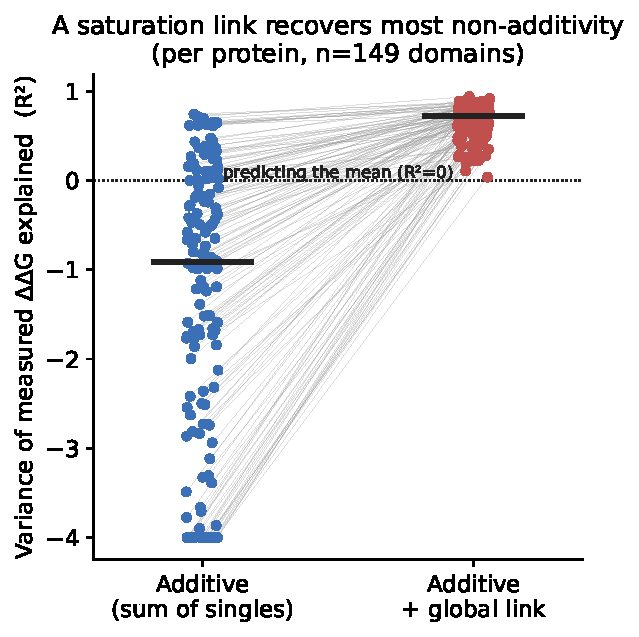
\includegraphics[width=0.86\columnwidth]{fig2_three_layer_r2.pdf}
  \caption{Per-protein variance of measured stability explained, additive
  baseline (left) vs.\ additive$+$global saturation link (right), across 149
  Megascale domains. A single monotonic link per protein recovers most of the
  non-additivity; bars are medians. Regenerated by
  \texttt{scripts/build\_epistasis\_figures.py} from the committed atlas.}
  \label{fig:three_layer}
\end{figure}

\begin{figure}[t]
  \centering
  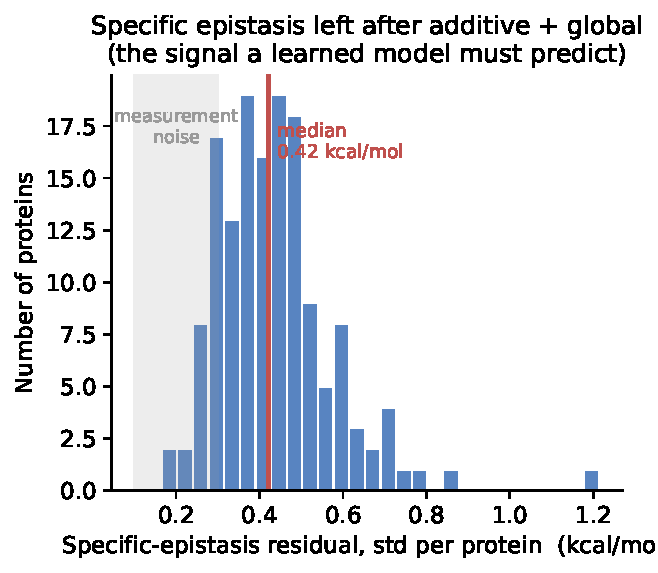
\includegraphics[width=0.86\columnwidth]{fig3_specific_epistasis.pdf}
  \caption{Distribution of specific-epistasis residual magnitude (per-protein
  standard deviation, kcal/mol) after removing the additive and global layers.
  The median ($0.42$ kcal/mol, red) sits above the illustrative measurement-scatter
  band (grey): the signal a learned model must predict.}
  \label{fig:specific}
\end{figure}

\begin{table}[t]
  \centering
  \caption{Three-layer decomposition over the Megascale double-mutant corpus
  (149 domains, 131{,}062 doubles). Source:
  \texttt{outputs/epistasis/decomposition\_summary.json}.}
  \label{tab:decomp}
  \small
  \begin{tabular}{lr}
    \toprule
    Quantity & Value \\
    \midrule
    Proteins / double mutants & 149 / 131{,}062 \\
    Median $R^2$, additive baseline & $-0.91$ \\
    Median $R^2$, additive $+$ global link & $0.72$ \\
    Proteins with additive $R^2 < 0$ & 72\% \\
    Median specific-epistasis std (kcal/mol) & $0.42$ \\
    Median specific variance share & 28\% \\
    Proteins with specific share $> 10\%$ & 98\% \\
    \bottomrule
  \end{tabular}
\end{table}

\subsection{Functional epistasis is invisible to zero-shot PLMs}
\label{sec:results-zs}

The stability result above is the setting where zero-shot PLMs do best, because
naturalness is coupled to stability. Even there, the zero-shot DPLM PLL epistasis
score (\cref{eq:zs}) is only a weak predictor of measured specific epistasis: over
30 Megascale domains (15{,}000 double mutants), its median per-protein Spearman
with the specific-epistasis residual is $0.25$ (overall Spearman $0.23$), and it
clears $\spearman > 0.2$ for only 60\% of proteins (\cref{tab:zeroshot},
\cref{fig:headroom}). This is
the ceiling for a label-free PLM epistasis score, and it is already modest in the
most favorable regime; the functional assays are the opposite regime. On GB1
IgG-binding (Olson) and GFP fluorescence (Sarkisyan), the same zero-shot DPLM PLL
correlation against measured specific epistasis collapses to essentially zero:
Spearman $0.021$ on GB1 and $0.005$ on GFP (\cref{tab:model1}, ``zero-shot''
column). Zero-shot PLM epistasis is therefore a stability-coupled signal that does
\emph{not} transfer to function -- it is, on these functional assays, no better
than chance. These two numbers are the
\texttt{model1\_\{GB1\_Olson,GFP\}\_summary.json:zeroshot\_spearman} keys, and they
are the floor any learned model must beat.

\begin{table}[t]
  \centering
  \caption{Zero-shot DPLM pseudo-log-likelihood epistasis (\cref{eq:zs}) vs.\
  measured specific epistasis on Megascale stability doubles -- the regime most
  favorable to a label-free PLM score, where naturalness and the assay are most
  coupled. Even here the zero-shot score is weak. Source:
  \texttt{outputs/epistasis/headroom\_summary.json}.}
  \label{tab:zeroshot}
  \small
  \begin{tabular}{lr}
    \toprule
    Quantity & Value \\
    \midrule
    Proteins / doubles scored & 30 / 15{,}000 \\
    Median per-protein Spearman & $0.25$ \\
    Overall Spearman & $0.23$ \\
    Proteins with per-protein $\spearman > 0.2$ & 60\% \\
    \bottomrule
  \end{tabular}
\end{table}

\begin{figure}[t]
  \centering
  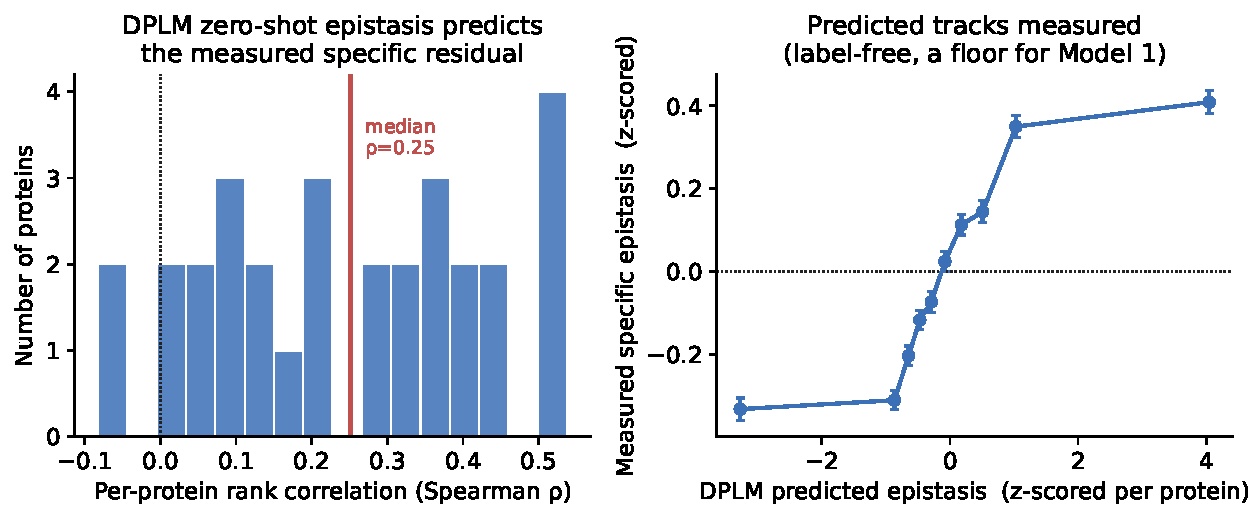
\includegraphics[width=\columnwidth]{fig4_headroom_dplm.pdf}
  \caption{Zero-shot DPLM PLL epistasis on Megascale stability doubles -- the
  regime most favorable to a label-free score. Left: distribution of per-protein
  Spearman against the specific-epistasis residual (median $0.25$, red). Right:
  binned measured residual vs.\ the zero-shot prediction (both z-scored per
  protein) -- the score tracks the residual but only weakly, a modest floor for
  the trained model. Regenerated by
  \texttt{scripts/build\_epistasis\_figures.py -{}-from-committed} from the
  committed \texttt{outputs/epistasis/headroom\_dplm.parquet}.}
  \label{fig:headroom}
\end{figure}

\subsection{Model 1: learned epistasis is predictable from DPLM representations}
\label{sec:results-model12}

The same residual that is invisible to the zero-shot score is, however,
\emph{predictable} from DPLM's internal representations. A pairwise coupling head
(\cref{sec:model1}) trained on each assay and evaluated out-of-fold lifts the
held-out-double Spearman from the near-zero zero-shot floor to $0.36$ on GB1 and
$0.14$ on GFP (\cref{tab:model1}, \cref{fig:model1}) -- a $+0.34$ and $+0.13$ gain
over zero-shot. Bootstrapping the held-out doubles ($2{,}000$ resamples) puts the
Model 1 Spearman at $0.36$ (95\% CI $[0.34, 0.38]$) on GB1 and $0.14$
($[0.12, 0.16]$) on GFP, while the zero-shot floor stays at $0.02$
($[0.00, 0.04]$) and $0.005$ ($[-0.01, 0.02]$, a CI that includes zero -- the
zero-shot score is statistically indistinguishable from chance on GFP function);
the paired-resample gain over zero-shot is significant on both assays
(95\% CI $[0.31, 0.36]$ and $[0.11, 0.16]$, both excluding zero). Source:
\texttt{outputs/epistasis/model1\_ci.json}.
The harder held-out-\emph{position} split, where every double at the test
residues is removed so the head must place couplings at positions it never saw
during training, still clears the floor ($0.12$ on GB1, $0.08$ on GFP); the same
bootstrap puts these at $0.12$ (95\% CI $[0.10, 0.14]$) and $0.08$
($[0.06, 0.10]$), both excluding zero, so even this cross-position transfer is
significantly above chance. Because
the head consumes only DPLM hidden states and representation shifts, never residue
indices, the recovered signal is genuinely carried in the representation rather
than memorized from position identity. Both rows are derived from the committed
out-of-fold predictions in \texttt{outputs/epistasis/model1\_oof\_\{GB1\_Olson,GFP\}.csv}.

\begin{table}[t]
  \centering
  \caption{Model 1 (pairwise coupling head over DPLM-650M representations) vs.\ the
  zero-shot DPLM PLL floor, Spearman against measured specific epistasis,
  out-of-fold. ``Doubles'' = held-out double mutants; ``Position'' = held-out
  residue positions (the harder transfer). Source:
  \texttt{outputs/epistasis/model1\_oof\_\{GB1\_Olson,GFP\}.csv} and the matching
  \texttt{model1\_*\_summary.json}.}
  \label{tab:model1}
  \small
  \begin{tabular}{lccc}
    \toprule
    Assay & Zero-shot & Model 1 (Doubles) & Model 1 (Position) \\
    \midrule
    GB1 (Olson) & $0.021$ & $0.36$ & $0.12$ \\
    GFP (Sarkisyan) & $0.005$ & $0.14$ & $0.08$ \\
    \bottomrule
  \end{tabular}
\end{table}

\begin{figure}[t]
  \centering
  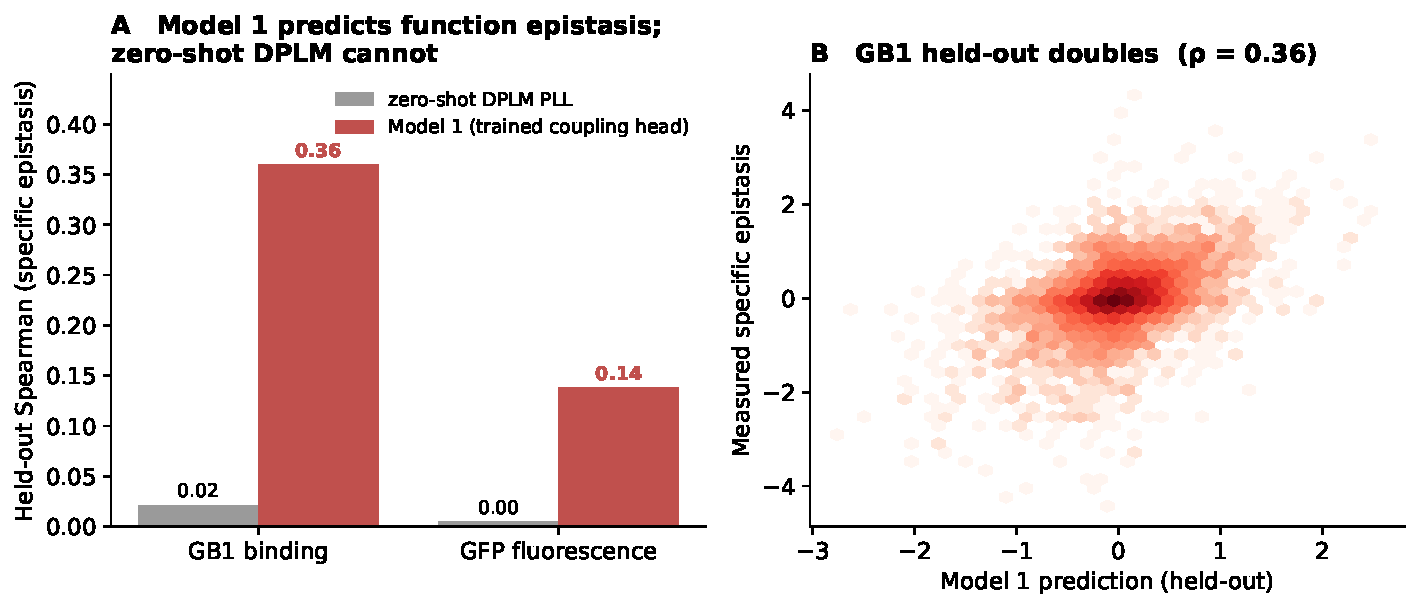
\includegraphics[width=\columnwidth]{fig8_model1_function.pdf}
  \caption{Model 1 predicts functional specific epistasis where the zero-shot
  score cannot. \textbf{A:} held-out Spearman, zero-shot DPLM PLL (grey) vs.\ the
  trained coupling head (red), on GB1 binding and GFP fluorescence. \textbf{B:}
  Model 1 out-of-fold prediction vs.\ measured specific epistasis on held-out GB1
  doubles ($\spearman = 0.36$). Regenerated by
  \texttt{scripts/build\_model1\_figure.py} from the committed
  \texttt{outputs/epistasis/model1\_oof\_\{GB1\_Olson,GFP\}.csv}.}
  \label{fig:model1}
\end{figure}

\subsection{Model 2: ranking by predicted epistasis finds gain-of-function}
\label{sec:results-model2}

On the 12{,}000 held-out GB1 double mutants, we form the design pool from the
additively-mediocre candidates (those below the median additive prediction, where
the additive model rates everything roughly equal) and select the top $10\%$ by
each reward. Measured binding is the ProteinGym DMS score for the Olson GB1
assay -- a dimensionless log-scale binding-enrichment value -- so the lifts
below are on that log scale. Ranking by Model 1's predicted specific epistasis
lifts the mean measured binding of the selection by $+1.09$ over the pool,
recovering most of the $+1.62$ oracle lift available to a perfect epistasis ranker
(\cref{tab:model2}). The standard PLM-as-reward design baseline -- best-of-$N$
reranking by the zero-shot DPLM PLL epistasis -- does \emph{worse than random
selection} from the pool ($-0.22$ lift), because that score is essentially blind
to functional epistasis (\cref{tab:model1}). The matched-additive control closes
the loop: within deciles of the additive prediction, where additive value is held
fixed, the median Spearman between predicted and measured specific epistasis is
$0.28$ (10 bins) -- by construction, signal the additive model cannot access, so
the recovered gain is genuine epistasis rather than relearned additivity
(\cref{fig:model2}). Bootstrapping the held-out doubles ($2{,}000$ resamples)
makes these significant: the matched-additive control Spearman is $0.28$
(95\% CI $[0.24, 0.31]$, excluding zero), the Model 1 design lift is $+1.09$
($[0.99, 1.20]$), and -- on the same resample -- Model 1's lift exceeds the
zero-shot rerank lift by $+1.31$ ($[1.17, 1.44]$), so ranking by predicted
epistasis significantly beats the PLM-as-reward baseline. All numbers derive from
the committed \texttt{outputs/epistasis/model2\_oof\_GB1.csv} and
\texttt{model2\_ci.json}.

\begin{table}[t]
  \centering
  \caption{Model 2 design on held-out GB1 doubles ($n=12{,}000$): mean measured
  binding (log-scale ProteinGym DMS score, dimensionless) of the top $10\%$
  selected from the additively-mediocre pool by each reward, and the lift over
  the additive pool mean. Ranking by Model 1's predicted
  epistasis recovers gain-of-function combinations the additive model rates equal;
  best-of-$N$ reranking by the zero-shot DPLM PLL reward is worse than random.
  Source: \texttt{outputs/epistasis/model2\_oof\_GB1.csv} and
  \texttt{model2\_GB1\_summary.json}.}
  \label{tab:model2}
  \small
  \begin{tabular}{lcc}
    \toprule
    Selection rule & Top-10\% binding & Lift \\
    \midrule
    Additive (pool mean) & $-3.62$ & $0.00$ \\
    Best-of-$N$ rerank (zero-shot DPLM PLL) & $-3.84$ & $-0.22$ \\
    Model 1 (predicted epistasis) & $-2.53$ & $+1.09$ \\
    Oracle (true epistasis) & $-2.00$ & $+1.62$ \\
    \bottomrule
  \end{tabular}
\end{table}

\begin{figure}[t]
  \centering
  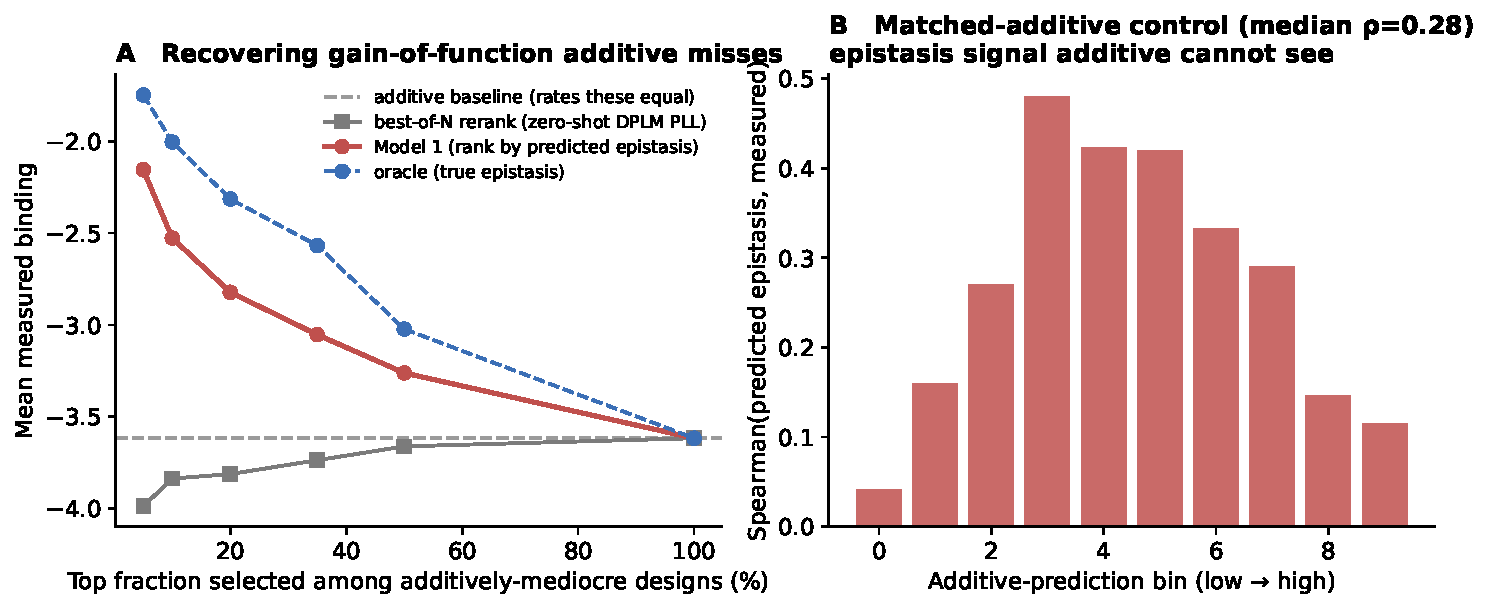
\includegraphics[width=\columnwidth]{fig9_model2_design.pdf}
  \caption{\textbf{Model 2 design.} (A) Mean measured binding of the top fraction
  selected from the additively-mediocre GB1 pool: ranking by Model 1's predicted
  epistasis (red) recovers gain-of-function combinations the additive baseline
  (grey) rates equal and best-of-$N$ reranking by the zero-shot DPLM PLL reward
  (grey squares) cannot find, approaching the oracle (blue). (B) Matched-additive
  control: within-bin Spearman between predicted and measured specific epistasis
  across additive-prediction deciles. Regenerates from
  \texttt{outputs/epistasis/model2\_oof\_GB1.csv} via
  \texttt{scripts/model2\_design.py}.}
  \label{fig:model2}
\end{figure}

\subsection{Cross-protein generalization}
\label{sec:results-e2e}

The end-to-end LoRA fine-tune (\cref{sec:e2e}) is trained on the double mutants of
124 Megascale stability domains and evaluated on the 25 held-out domains that
contribute no training examples. With rank-64 adapters (12.9M trainable
parameters) and 10 epochs, it reaches a median per-held-out-protein Spearman of
$0.33$ (mean $0.33$) between predicted and measured specific epistasis, clearing
$\spearman > 0.2$ for 80\% of held-out domains (\cref{tab:e2e}). This exceeds the
zero-shot DPLM PLL reference of $0.25$ -- the median per-protein Spearman of the
label-free score on the Megascale stability corpus (\cref{sec:results-zs},
\cref{tab:zeroshot}), the same specific-epistasis target and metric. The learned
$0.33$ is achieved \emph{on 25 proteins the head never saw}: the epistasis skill
learned across proteins transfers to new ones rather than being memorized per
protein. The $0.25$ is the corpus-level zero-shot ceiling for this regime, not a
zero-shot score re-measured on these exact held-out domains; because the zero-shot
baseline uses no training data, train/test overlap does not affect it, and a
per-held-out-protein zero-shot control would only sharpen the comparison -- we leave
it to future work (\cref{sec:limitations}). The transfer is demonstrated on
stability because that is the only corpus with enough proteins for a
held-out-protein split; transferring the \emph{functional} skill across proteins is
the analogous open problem (\cref{sec:limitations}). The $0.33$, mean, and $80\%$
numbers are read from the committed \texttt{outputs/epistasis/e2e\_results.json}; the
$0.25$ reference is the committed headroom baseline
(\texttt{outputs/epistasis/headroom\_summary.json}).

\begin{table}[t]
  \centering
  \caption{Cross-protein generalization of the end-to-end LoRA fine-tune,
  evaluated on the 25 held-out Megascale proteins (no training examples).
  The reference is the zero-shot DPLM PLL median per-protein Spearman on the
  Megascale stability corpus (\cref{tab:zeroshot}) -- the same specific-epistasis
  target and metric, a corpus-level ceiling, not re-measured on these 25 held-out
  domains. Source: \texttt{outputs/epistasis/e2e\_results.json}; the zero-shot
  reference is \texttt{outputs/epistasis/headroom\_summary.json}.}
  \label{tab:e2e}
  \begin{tabular}{lc}
    \toprule
    Held-out generalization (25 proteins) & Spearman \\
    \midrule
    Median per-held-out-protein   & $0.33$ \\
    Mean per-held-out-protein     & $0.33$ \\
    Fraction with $\spearman>0.2$ & $0.80$ \\
    \midrule
    Zero-shot DPLM PLL reference  & $0.25$ \\
    \bottomrule
  \end{tabular}
\end{table}

\section{Limitations}
\label{sec:limitations}

Our strongest, fully-committed result is the stability decomposition; the
functional prediction and design results rest on a small number of assays with
complete combinatorial coverage (GB1, GFP), chosen precisely because every design
is measurable, and may not represent all functional landscapes. The cross-protein
transfer result (\cref{sec:results-e2e}) is likewise demonstrated on the Megascale
stability corpus, the only corpus here with enough proteins for a held-out-protein
split; an analogous held-out-protein test of \emph{functional} epistasis transfer
would require many more combinatorial functional assays than currently exist, so
cross-protein transfer of the functional skill specifically remains future work.
The global layer is a per-protein monotonic link fit on the same assay it
explains; we therefore report specific epistasis only as a held-out residual,
never as in-sample fit.
Model 1's held-out-position transfer is the hardest regime and is expected to be
weak. We do not make a generative design claim and therefore do not benchmark
against discrete-diffusion guidance \citep{gruver2023protein,nisonoff2025unlocking}
or reward-guided refinement \citep{wang2025drakes,li2024svdd}; Model 2 is a
ranking policy over measurable candidates. Finally, all results are
\emph{in silico}: no wet-lab validation of designed variants is included.

\section{Conclusion}
\label{sec:conclusion}

Multi-mutant protein function decomposes into additive, global, and specific
epistasis. The specific layer is large and ubiquitous, is the only part under
which combinations beat the additive expectation, and -- unlike global epistasis
on stability -- is invisible to zero-shot protein language models. We show it is
nonetheless predictable from a PLM's internal representations, enough to design
gain-of-function combinations an additive model cannot find, and we test whether
that skill transfers across proteins. Treating specific epistasis as the explicit
learning target, rather than raw fitness, turns ``do PLMs know epistasis?'' into a
clean, held-out, design-relevant question.

\bibliography{epistasis}
\bibliographystyle{icml2025}

\end{document}
